\documentclass{beamer}
\mode<presentation>
\usetheme{CambridgeUS}
\usepackage[russian]{babel}
\usepackage[utf8]{inputenc}
\usepackage[T2A]{fontenc}
\usepackage{sansmathaccent}

\usepackage{verbatim}
\usepackage{alltt}

\pdfmapfile{+sansmathaccent.map}
\title[Язык C]{Низкоуровневый ввод-вывод, часть 5}
\author{Наумов Д.А., доц. каф. КТ}
\date[02.10.2019] {Операционные системы и системное программное обеспечение, 2019}

\begin{document}

%ТИТУЛЬНЫЙ СЛАЙД
\begin{frame}
  \titlepage
\end{frame}
  
%СОДЕРЖАНИЕ ЛЕКЦИИ
\begin{frame}
  \frametitle{Содержание лекции}
  \tableofcontents  
\end{frame}

\section{Файловый ввод-вывод}

\subsection{Открытие файлов}

\begin{frame}{Файловый ввод-вывод}
\begin{itemize}
\item Ядро поддерживает попроцессный список открытых файлов, называемый файловой таблицей. 
\item Таблицы индексируется с помощью неотрицательных целых чисел, называемых файловыми дескрипторами (часто они именуются сокращенно jd). 
\item Каждая запись в списке содержит информацию об открытом файле, в частности указатель на хранимую в памяти копию файлового дескриптора и ассоциированных с ним метаданных.
\item К метаданным относятся, в частности, файловая позиция и режимы доступа. 
\end{itemize}
\end{frame}

\begin{frame}{Стандартные дескрипторы}
\begin{itemize}
\item Каждый процесс традиционно имеет не менее трех открытых файловых дескрипторов: 0, 1 и 2. 
\item Файловый дескриптор 0 соответствует стандартному вводу (stdin), дескриптор 1 — стандартному выводу (stdout), дескриптор 2 — стандартной ошибке (stderr).
\item Библиотека С не ссылается непосредственно на эти целые числа, а предоставляет препроцессорные определения STDIN\_FILENO, STDOUT\_FILENO и STDERR\_FILENO для каждого из вышеописанных вариантов соответственно. 
\item Как правило, stdin подключен к терминальному устройству ввода (обычно это пользовательская клавиатура), а stdout и stderr — к дисплею терминала. 
\end{itemize}
\end{frame}

\begin{frame}{Системный вызов open()}
Открытие файла и получение файлового дескриптора осуществляются с помощью системного вызова open():
\begin{figure}[h]
\centering
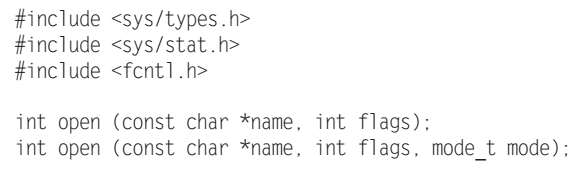
\includegraphics[scale=0.6]{images/lec06-pic01.png}
\end{figure}
Системный вызов open() ассоциирует файл, на который указывает имя пути name
с файловым дескриптором, возвращаемым в случае успеха. В качестве файловой  позиции указывается его начало (нуль), и файл открывается для доступа в соответствии с заданными флагами (параметр flags).
\end{frame}

\begin{frame}{Флаги для открытия файла}
\begin{itemize}
\item Аргумент flags — это поразрядное ИЛИ, состоящее из одного или нескольких флагов, определяющее режим доступа к файлу. 
\item Режим доступа может иметь одно из следующих значений: O\_RDONLY, O\_WRONLY или O\_RDWR.
\end{itemize}
\begin{figure}[h]
\centering
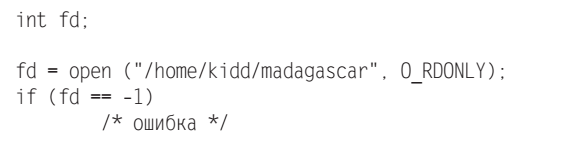
\includegraphics[scale=0.6]{images/lec06-pic02.png}
\end{figure}
\begin{itemize}
\item Если файл открыт только для чтения, в него невозможно что­либо записать, и наоборот. 
\item Процесс, осуществляющий системный вызов open(), должен иметь права, чтобы получить запрашиваемый доступ. 
\end{itemize}
\end{frame}

\begin{frame}{Открытие файла}
Некоторые дополнительные флаги аргумента flags для изменения поведения open(). 
\begin{itemize}
\item O\_APPEND. Режим дозаписи - перед каждым актом записи файловая позиция будет обновляться и устанавливаться в текущий конец файла.
\item O\_CREAT. Если файл, обозначаемый именем name, не существует, то ядро создаст
его. 
\item O\_TRUNC. Если файл уже существует, является обычным файлом и заданные для
него флаги допускают запись, то файл будет усечен до нулевой длины. 
\end{itemize}
\end{frame}

\begin{frame}{Открытие файла}
Дополнительные флаги аргумента flags для изменения поведения open(). 
\begin{itemize}
\item O\_ASYNC. Когда указанный файл станет доступным для чтения или записи, генерируется специальный сигнал (по умолчанию SIGIO). Этот флаг может использоваться только при работе с FIFO, каналами, сокетами и терминалами, но не
с обычными файлами.
\item O\_SYNC. Файл будет открыт для синхронного ввода­вывода. Никакие операции
записи не завершатся, пока данные физически не окажутся на диске. 
\end{itemize}
\end{frame}

\begin{frame}{Права доступа создаваемых файлов}
Аргумент mode требуется, если задан флаг O\_CREAT. 
\begin{figure}[h]
\centering
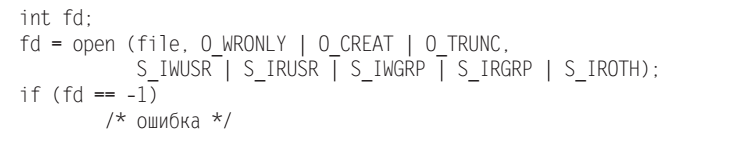
\includegraphics[scale=0.6]{images/lec06-pic04.png}
\end{figure}
\begin{itemize}
\item при создании файла аргумент mode задает права доступа к этому новому файлу;
\item режим доступа не проверяется при данном конкретном открытии файла;
\item аргумент mode является UNIX-­последовательностью битов, регламентирующей доступ.
\end{itemize}
\end{frame}

\begin{frame}{Функция creat()}
Комбинация O\_WRONLY | O\_CREAT | O\_TRUNC настолько распространена, что существует
специальный системный вызов, обеспечивающий именно такое поведение:. 
\begin{figure}[h]
\centering
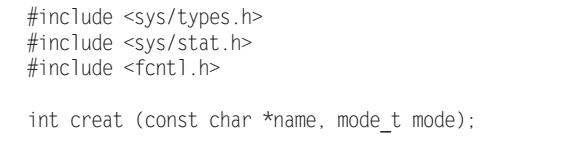
\includegraphics[scale=0.6]{images/lec06-pic05.png}
\end{figure}
В большинстве архитектур Linux creat() является системным вызовом, хотя
его можно легко реализовать и в пользовательском пространстве:
\begin{figure}[h]
\centering
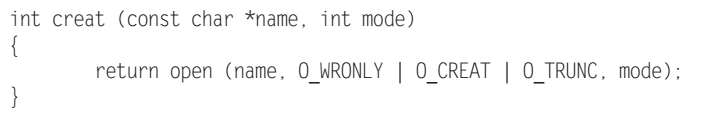
\includegraphics[scale=0.6]{images/lec06-pic06.png}
\end{figure}
При ошибке open() и creat() возвращают –1 и устанавливают errno.
\end{frame}

\subsection{Чтение данных}

\begin{frame}{Системный вызов read()}
\begin{figure}[h]
\centering
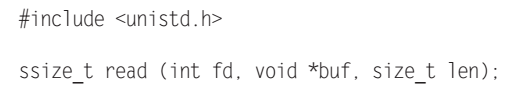
\includegraphics[scale=0.6]{images/lec06-pic07.png}
\end{figure}
\begin{itemize}
\item Каждый вызов считывает не более len байт в памяти, на которые содержится
указание в buf. 
\item Считывание происходит с текущим значением смещения, в файле,
указанном в fd. 
\item При успешном вызове возвращается количество байтов, записанных
в buf. 
\item При ошибке вызов возвращает -1 и устанавливает errno. 
\item Файловая позиция продвигается в зависимости от того, сколько байтов было считано с fd. 
\item Если объект, указанный в fd, не имеет возможности позиционирования (например, это файл символьного устройства), то считывание всегда начинается с «текущей» позиции.
\end{itemize}
\end{frame}

\begin{frame}{Системный вызов read()}
\begin{figure}[h]
\centering
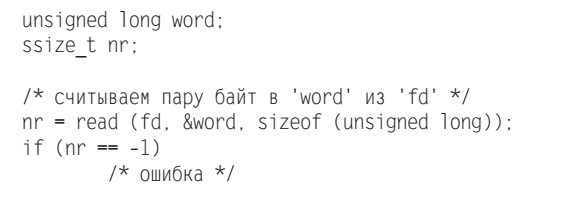
\includegraphics[scale=0.6]{images/lec06-pic08.png}
\end{figure}
\begin{itemize}
\item вызов может вернуться, считав не все байты из len; 
\item могут возникнуть ошибки, требующие исправления, но не проверяемые и не обрабатываемые в коде.
\end{itemize}
\end{frame}

\begin{frame}{Последствия вызова read()}
\begin{itemize}
\item вызов возвращает значение, равное len. Все len считанных байтов сохраняются
в buf. 
\item вызов возвращает значение, меньшее чем len, но большее чем нуль. Считанные
байты сохраняются в buf. Ошибка возникает в середине процесса, становится доступно значение, большее 0, но меньшее len. Конец файла был достигнут ранее, чем было прочитано заданное количество байтов. При повторном вызове (в котором соответствующим образом обновлены значения len и buf) оставшиеся байты будут считаны в оставшуюся часть буфера либо укажут на причину проблемы.
\item Вызов возвращает 0. Это означает конец файла. Считывать больше нечего.
\item Вызов блокируется, поскольку в текущий момент данные недоступны. Этого не
происходит в неблокирующем режиме.
\end{itemize}
\end{frame}

\begin{frame}{Последствия вызова read()}
\begin{itemize}
\item Вызов возвращает –1, а errno присваивается EINTR. Это означает, что сигнал был получен прежде, чем были считаны какие­либо байты. Вызов будет повторен.
\item Вызов возвращает –1, а errno присваивается EAGAIN. Это означает, что вызов
блокировался потому, что в настоящий момент нет доступных данных, и запрос
следует повторить позже. Это происходит только в неблокирующем режиме.
\item Вызов возвращает –1, а errno присваивается иное значение, нежели EINTR или
EAGAIN. Это означает более серьезную ошибку. Простое повторение вызова в данном случае, скорее всего, не поможет.
\end{itemize}
\end{frame}

\begin{frame}{Считывание всех байт)}
\begin{figure}[h]
\centering
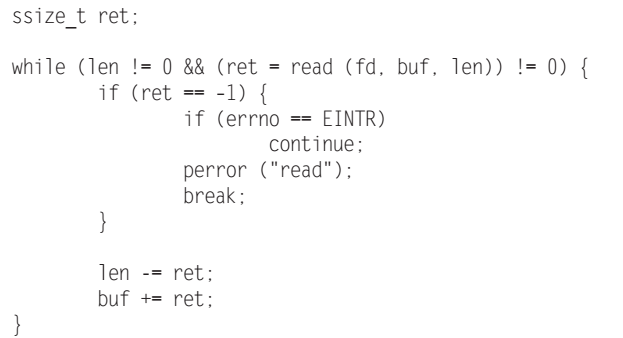
\includegraphics[scale=0.6]{images/lec06-pic09.png}
\end{figure}
\end{frame}

\begin{frame}{Неблокирующее считывание)}
\textbf{Неблокирующий ввод-вывод} - вызов read() не блокируется при отсутствии доступных данных, вместо этого - немедленный возврат вызова, указывающий, что данных действительно нет. 
\begin{figure}[h]
\centering
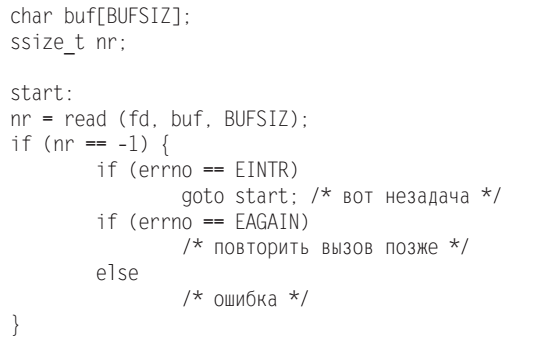
\includegraphics[scale=0.6]{images/lec06-pic10.png}
\end{figure}
\end{frame}

\subsection{Запись данных}

\begin{frame}{Системный вызов write()}
\begin{figure}[h]
\centering
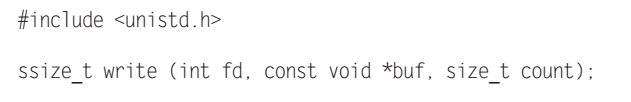
\includegraphics[scale=0.6]{images/lec06-pic11.png}
\end{figure}
\begin{itemize}
\item при вызове write() записывается некоторое количество байтов, меньшее или
равное тому, что указано в count. 
\item запись начинается с buf, установленного в текущую файловую позицию. 
\item при успешном выполнении возвращается количество записанных байтов, а файловая позиция обновляется соответственно. 
\item при ошибке возвращается -1 и устанавливается соответствующее значение errno.
\end{itemize}
\end{frame}

\begin{frame}{Простейшиый пример использования}
\begin{figure}[h]
\centering
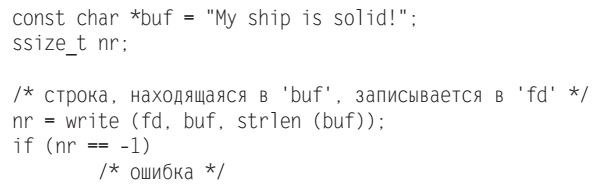
\includegraphics[scale=0.6]{images/lec06-pic12.png}
\end{figure}
\end{frame}

\begin{frame}{Проверка всех ошибок}
\begin{figure}[h]
\centering
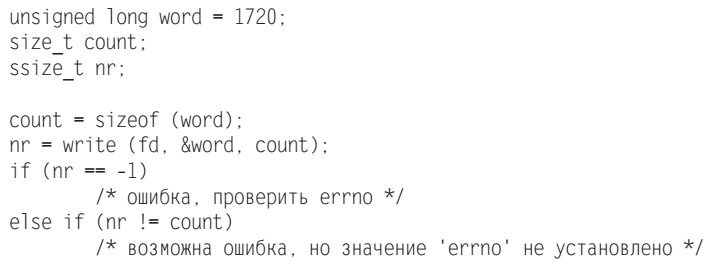
\includegraphics[scale=0.6]{images/lec06-pic13.png}
\end{figure}
\end{frame}

\begin{frame}{Режимы записи и ошибки}
Режим дозаписи: 
\begin{itemize}
\item Когда дескриптор fd открывается в режиме дозаписи (с флагом O\_APPEND), запись начинается не с текущей позиции дескриптора файла, а с точки, в которой в данный момент находится конец файла.
\end{itemize}
Неблокирующая запись: 
\begin{itemize}
\item Когда дескриптор fd открывается в неблокирующем режиме (с флагом O\_NONBLOCK),
а запись в том виде, в котором она выполнена, в нормальных условиях должна быть
заблокирована, системный вызов write() возвращает –1 и устанавливает errno в значение EAGAIN. Запрос следует повторить позже.
\end{itemize}
Если значение count превышает SSIZE\_MAX, то результат вызова write() не определен.
\end{frame}

\section{Синхронный ввод-вывод}
\begin{frame}{Синхронный ввод-вывод}
\begin{block}{fsync()}
Метод, позволяющий гарантировать, что данные окажутся на диске -  использовать системный вызов fsync().
\begin{figure}[h]
\centering
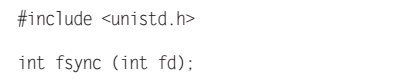
\includegraphics[scale=0.6]{images/lec06-pic14.png}
\end{figure}
\end{block}
\begin{itemize}
\item Вызов fsync() гарантирует, что все грязные данные, ассоциированные с конкретным файлом, на который отображается дескриптор fd, будут записаны на диск.
\item Файловый дескриптор fd должен быть открыт для записи. 
\item Вызов заносит на диск как данные, так и метаданные (цифровые отметки о времени создания файла и другие атрибуты).
\item Вызов fsync() не вернется, пока жесткий диск не сообщит, что все данные и метаданные оказались на диске.
\end{itemize}
\end{frame}

\begin{frame}{Коды ошибок fsync, fdatasync}
В случае успеха возвращается 0, в противном возвращается –1.

Устанавливается значение errno:
\begin{itemize}
\item EBADF -  указанный дескриптор файла не является допустимым дескриптором, открытым для записи;
\item EINVAL - указанный дескриптор файла отображается на объект, не поддерживающий синхронизацию;
\item EIO - при синхронизации произошла низкоуровневая ошибка ввода­вывода.
\end{itemize}
\end{frame}

\begin{frame}{Синхронный ввод-вывод}
\begin{block}{sync()}
обеспечивает синхронизацию всех буферов, имеющихся на диске
\begin{figure}[h]
\centering
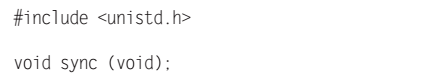
\includegraphics[scale=0.6]{images/lec06-pic15.png}
\end{figure}
\end{block}
\begin{itemize}
\item функция не имеет ни параметров, ни возвращаемого значения. 
\item функция всегда завершается успешно, и после ее возврата все буферы — содержащие как данные,
так и метаданные — гарантированно оказываются на диске.
\end{itemize}
\end{frame}

\begin{frame}{Флаг синхронизации}
Флаг O\_SYNC может быть передан вызову open(). Этот флаг означает, что все операции
ввода­вывода, осуществляемые с этим файлом, должны быть синхронизированы.
\begin{figure}[h]
\centering
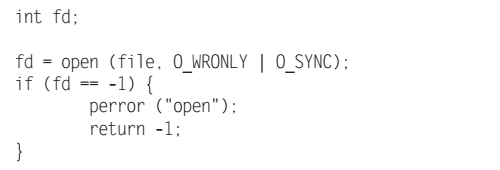
\includegraphics[scale=0.6]{images/lec06-pic16.png}
\end{figure}
\begin{itemize}
\item запросы на считывание синхронизированы \textbf{всегда}. 
\item вызовы write(), как правило, не синхронизируются.
\end{itemize}
Флаг O\_SYNC можно рассмотреть в следующем ключе: он принудительно выполняет неявный вызов fsync() после каждой операции write() перед возвратом вызова. 
\end{frame}

\section{Закрытие файлов}
\begin{frame}
Системный вызов close() - разорвать связь между дескриптором и файлом, который с ним ассоциирован
\begin{figure}[h]
\centering

\includegraphics[scale=0.6]{images/lec06-pic17.png}
\end{figure}
\begin{itemize}
\item close() отменяет отображение открытого файлового дескриптора fd и разрывает связь между файлом и процессом. 
\item ядро свободно может переиспользовать дескриптор как возвращаемое значение для последующих вызовов open() или creat(). 
\item успешное выполнение - возвращается 0, иначе -1. 
\end{itemize}
\begin{figure}[h]
\centering

\includegraphics[scale=0.6]{images/lec06-pic18.png}
\end{figure}
\begin{itemize}
\item Закрытие файла никак не связано с актом сбрасывания файла на диск. 
\end{itemize}
\end{frame}

\section{Позиционирование, усечение}
\begin{frame}
Системный вызов lseek() предназначен для установки в заданное значение файловой позиции конкретного файлового дескриптора. 
\begin{figure}[h]
\centering
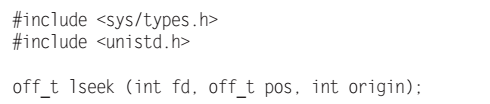
\includegraphics[scale=0.6]{images/lec06-pic19.png}
\end{figure}
Аргумент origin:
\begin{itemize}
\item SEEK\_CUR - текущая файловая позиция дескриптора fd установлена в его текущее
значение плюс pos. Последний может иметь отрицательное, положительное или
нулевое значение. Если pos равен нулю, то возвращается текущее значение
файловой позиции.
\item SEEK\_END - текущая файловая позиция дескриптора fd установлена в текущее
значение длины файла плюс pos, который может иметь отрицательное, положительное или нулевое значение. Если pos равен нулю, то смещение устанавливается в конец файла.
\end{itemize}
\end{frame}

\begin{frame}
Системный вызов lseek() предназначен для установки в заданное значение файловой позиции конкретного файлового дескриптора. 
\begin{figure}[h]
\centering
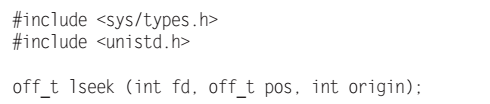
\includegraphics[scale=0.6]{images/lec06-pic19.png}
\end{figure}
Аргумент origin:
\begin{itemize}
\item SEEK\_SET - текущая файловая позиция дескриптора fd установлена в pos. Если
pos равен нулю, то смещение устанавливается в начало файла. 
\end{itemize}
\end{frame}

\begin{frame}{Системный выхов lseek()}
Файловая позиция дескриптора fd получает значение 1825:
\begin{figure}[h]
\centering
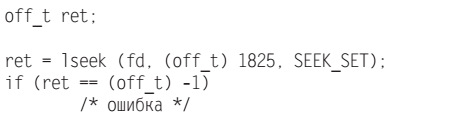
\includegraphics[scale=0.6]{images/lec06-pic20.png}
\end{figure}
\end{frame}

\begin{frame}{Системный выхов lseek()}
Установить файловую позицию дескриптора fd в конец файла:
\begin{figure}[h]
\centering
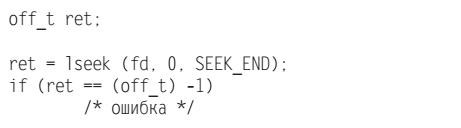
\includegraphics[scale=0.6]{images/lec06-pic21.png}
\end{figure}
\end{frame}

\begin{frame}{Системный выхов lseek()}
Вызов lseek() возвращает обновленную файловую позицию, поэтому его можно использовать для поиска текущей файловой позиции:
\begin{figure}[h]
\centering
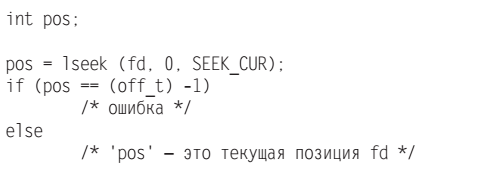
\includegraphics[scale=0.6]{images/lec06-pic22.png}
\end{figure}
\end{frame}

%\section{Внутренняя организация ядра}

\end{document}
